The High Performance Computing Consortium (HPCNY), supported by
the Empire State Development Division of Science, Technology and Innovation
(NYSTAR), is a multi-year effort to address the impediments listed in
Section~\ref{sec:impediments}.
HPCNY supports computational scientists to work directly with New York State
industry to apply massively parallel simulations on supercomputer systems.
Computational scientists are based at Rensselaer Polytechnic Institute,
University of Buffalo, SUNY Stoneybrook/Brookhaven National Lab, Icahn School of
Medicine at Mount Sinai, and Marist College.
Critical to the success of the computational scientists is the base
institution's faculty with extensive knowledge of high performance computing in
a broad range of application areas, existing industrial and software vendor
collaborations, and on-site HPC hardware systems programmers.

Industrial partners work with Rensselaer through HPCNY at the level needed to
address their computing requirements.
At one extreme are industrial partners that have the necessary technical
personnel, business case, and software to utilize available HPC hardware.
For these interactions an allocation on the Intel Xeon cluster and IBM
Blue Gene/Q at the Rensselaer Center for Computational Innovations (CCI) paired
with occasional help from systems programmers and computational scientist is
sufficient.

The more common cases are industrial partners that identify a computing need,
but face most of the impediments described in Section~\ref{sec:impediments}.
For these interactions the appropriate combination of computational scientists,
researchers, and software vendors are brought to bear on the problem.
In many cases the initial statement of the problem is of broad scope.
Thus, the first task then is to define a specific problem that includes the
relevant physical phenomena and geometric complexity.
Execution of this first problem demonstrates the computational and analytical
performance of the chosen HPC software technologies as well as the ability of
those technologies to integrate into simulation workflows accessible to the
industrial partners.
From a successful first problem demonstration the business case can be stated
and supported.
For the technical contact at the industrial partner the business case often
provides the necessary management level support to continue work with HPCNY
computational scientists to generalize the workflows for broader use.

While technical interactions proceed, HPCNY business administrators and
computational scientists work with the industrial partners to collect
economic impact statements and write press releases summarizing the
interactions.
Despite their non-technical nature, these materials are critical for the success
and growth of the consortium.
For NYSTAR they establish the return-on-investment needed to justify continued
funding from the state.
For other New York State companies they provide examples of prior success that
are often enough to motivate a first contact with HPCNY.

Companies typically understand that there is potential for HPC to improve their
competitive advantage but face some technical impediments.
In the following sections we describe how the technical impediments are
addressed for three industrial flow problems.
The first problem (Section~\ref{sec:nozzle}) is an example where we address
the limited fidelity and performance provided by a commercial CFD software suite
by coupling scalable and efficient mesh adaptation with a massively parallel,
open-source, CFD analysis component.
In the second problem (Section~\ref{sec:twinscrew}), simulating the flow of
a non-Newtonian fluid through a twin-screw extruder, we apply a similar approach,
but also address another critical bottleneck; the manual transfer of information
between the engineer and the software.
In a production environment, this transfer can be just as limiting to
productivity as a poorly performing flow solver, or a file-based transfer
between parallel components in a workflow.
Thus, for the extruder workflow we automated the process of executing the
workflow on remote parallel systems by defining a web-based gateway for job
submission and management.
In the third example problem (Section~\ref{sec:pumpdesign}), workflow
automation is again the focus.
For this workflow we automate the problem set up and execution steps required to
run an ensemble of simulations for studying pump design using a closed-source
CFD analysis framework.

\section{Micromechanical Device Analysis}\label{sec:nozzle}

Micromechanical device engineers at a New York State equipment manufacturer
study the design of a multi-phase flow system that is driven by a structural
boundary condition.  3D simulations use a commercial CFD software suite ran on in-house
multi-core workstations.
But, engineers typically run reduced fidelity 2D simulations due to the long
execution time of 3D simulations, limited computing resources, and finite design
periods.
In these simulations the fidelity is further reduced as the structure driving
the boundary condition is not influenced by the fluid flow.
Rensselaer computational scientists defined and demonstrated an end-to-end
workflow for guiding device design that uses the PHASTA
CFD~\cite{WhiJan01,phasta_github} suite of
tools for automated 3D parallel adaptive simulations~\cite{zhou2012unstructured}
that account for fluid-structure interactions.

\begin{figure} \centering
  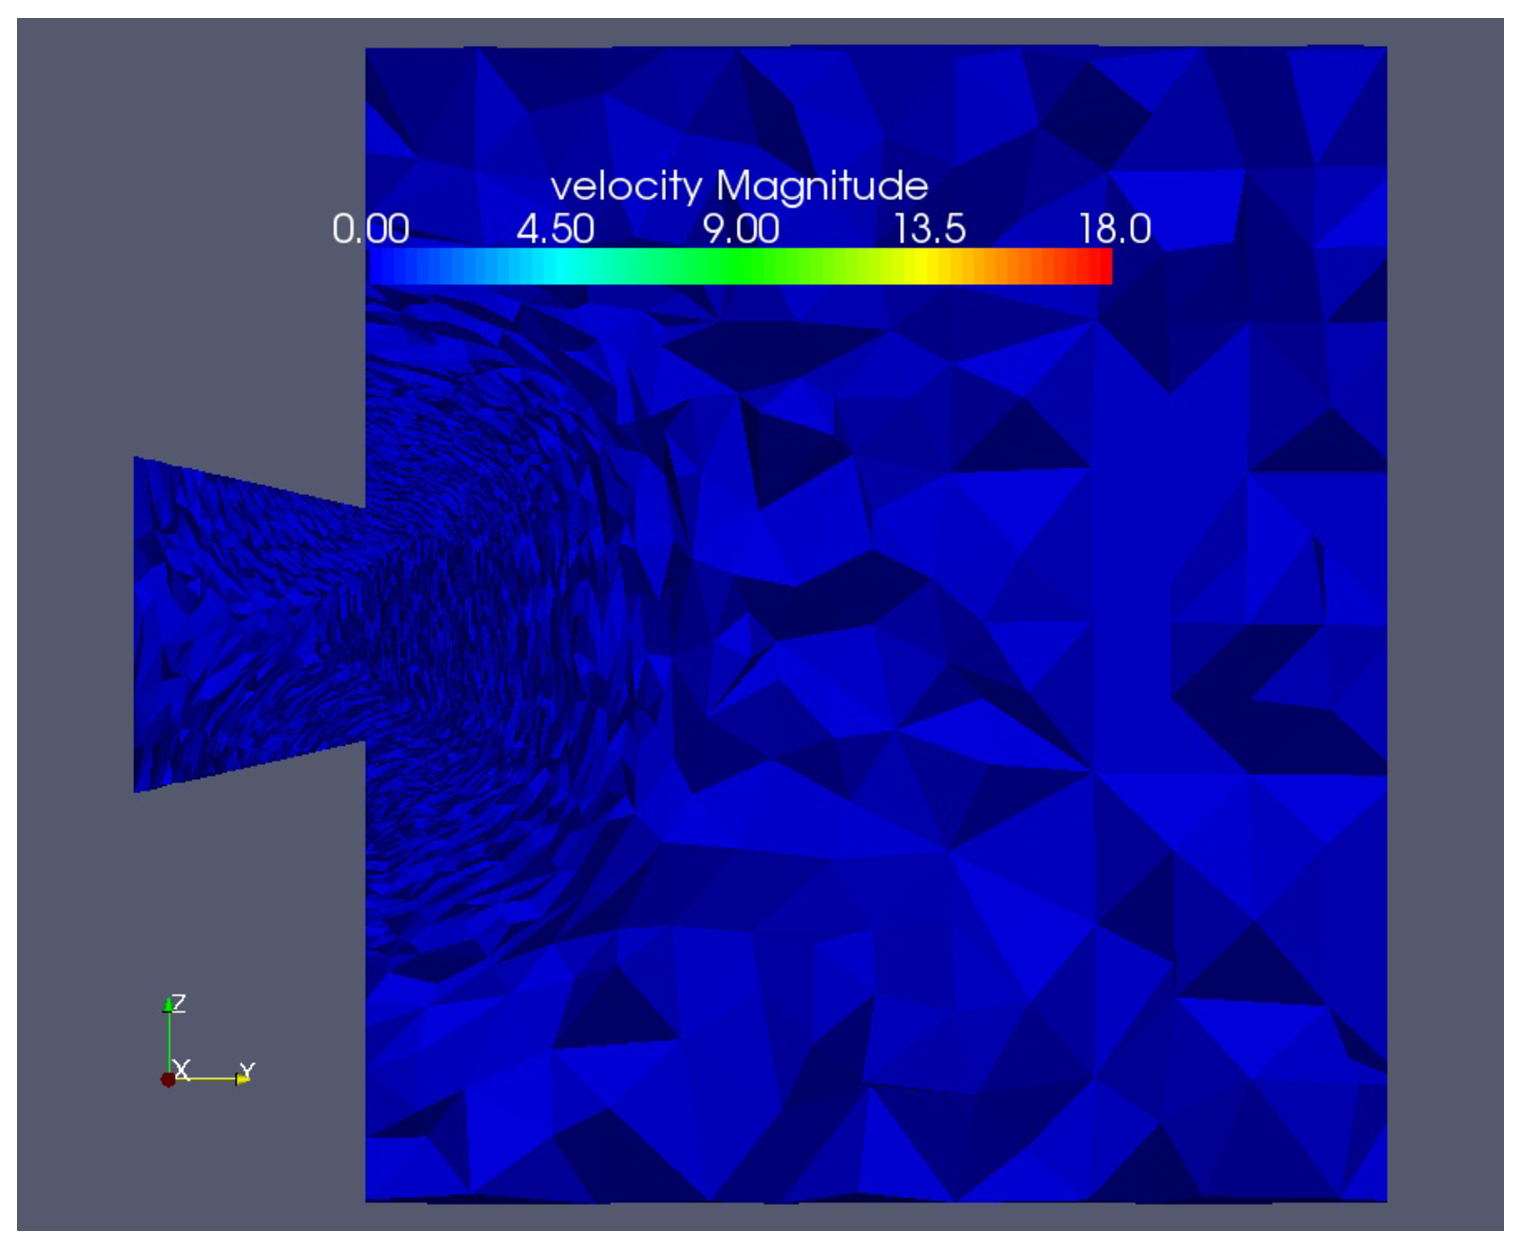
\includegraphics[width=0.49\textwidth]{figures/fig2a.eps}
  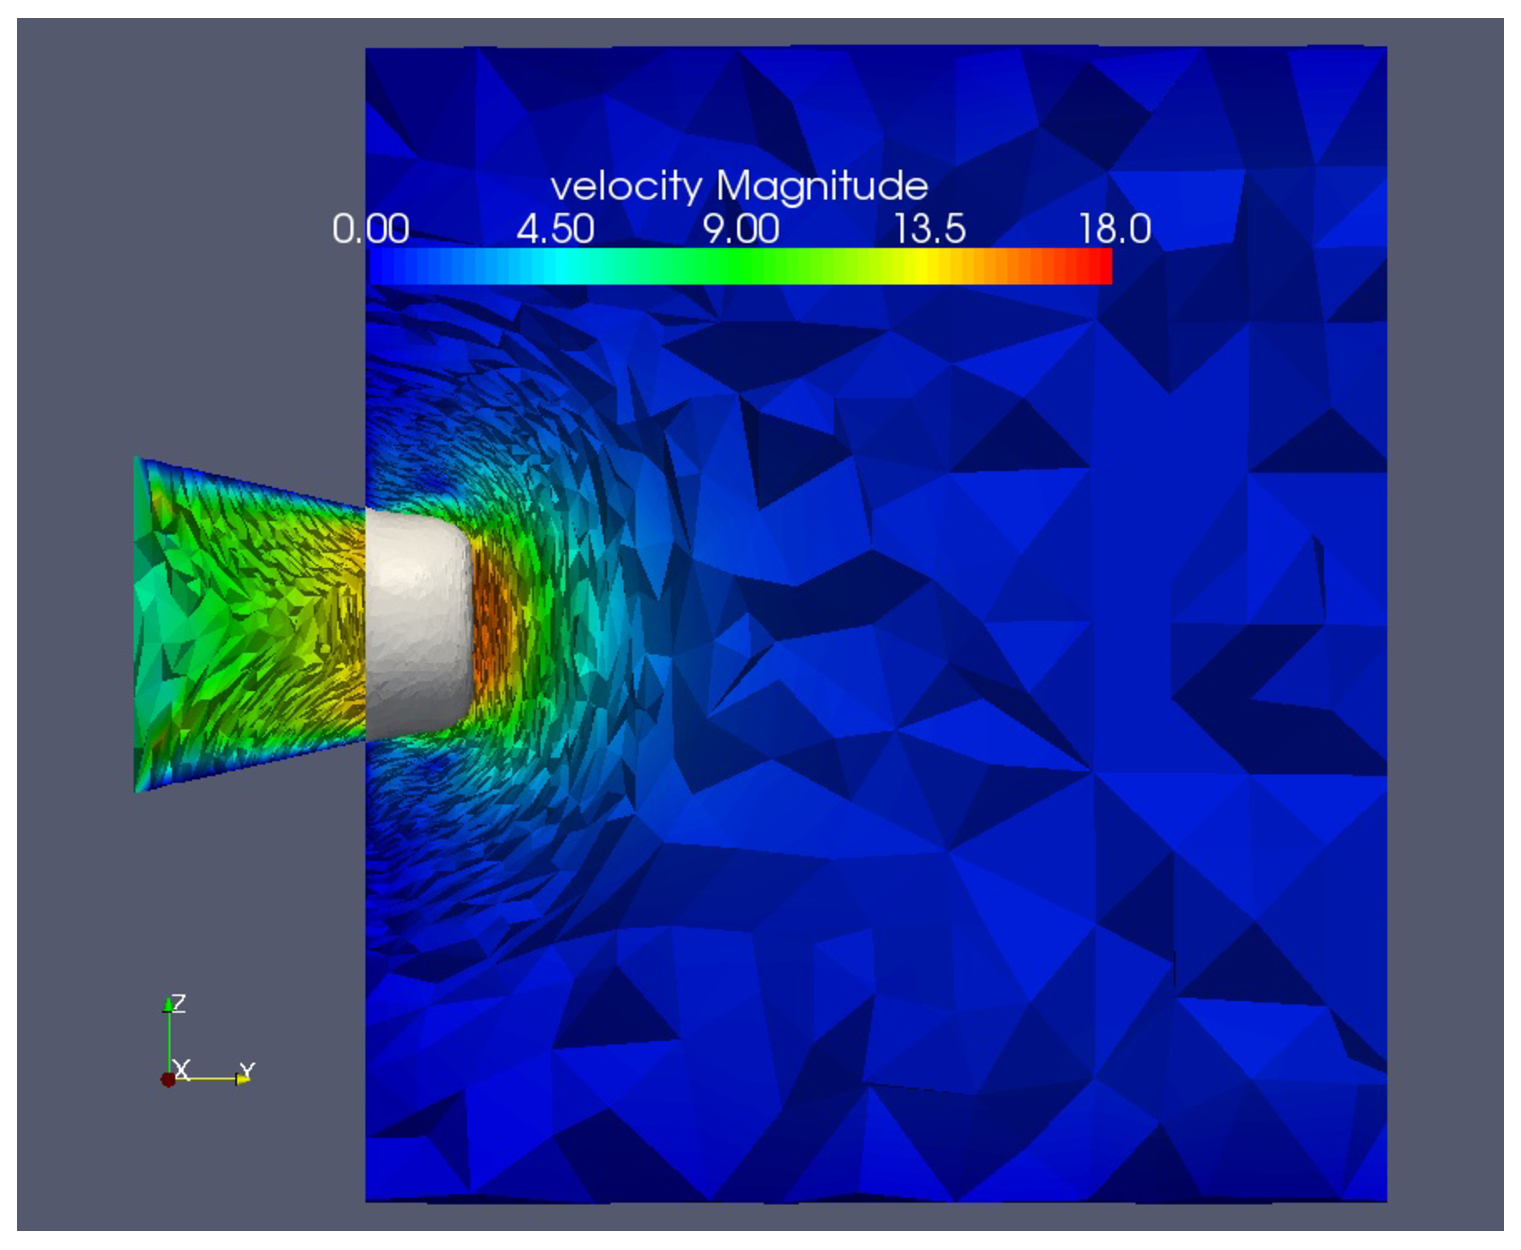
\includegraphics[width=0.49\textwidth]{figures/fig2b.eps}
  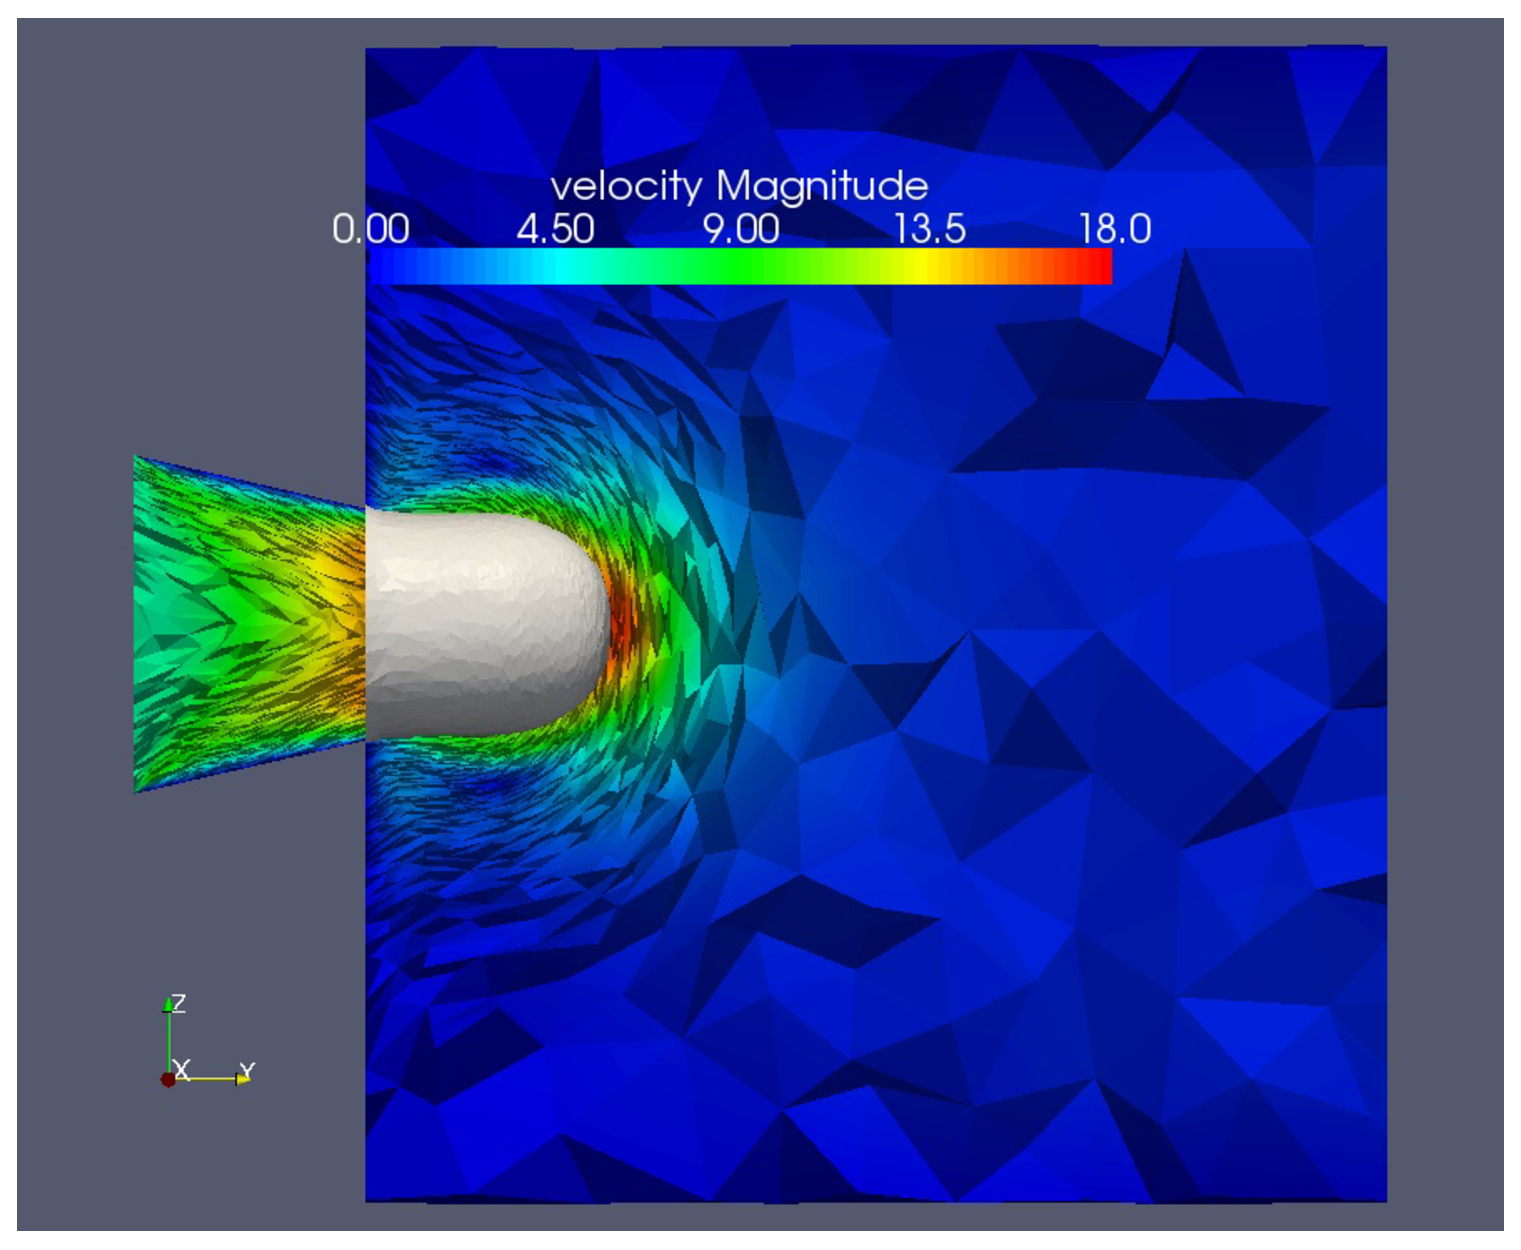
\includegraphics[width=0.49\textwidth]{figures/fig2c.eps}
  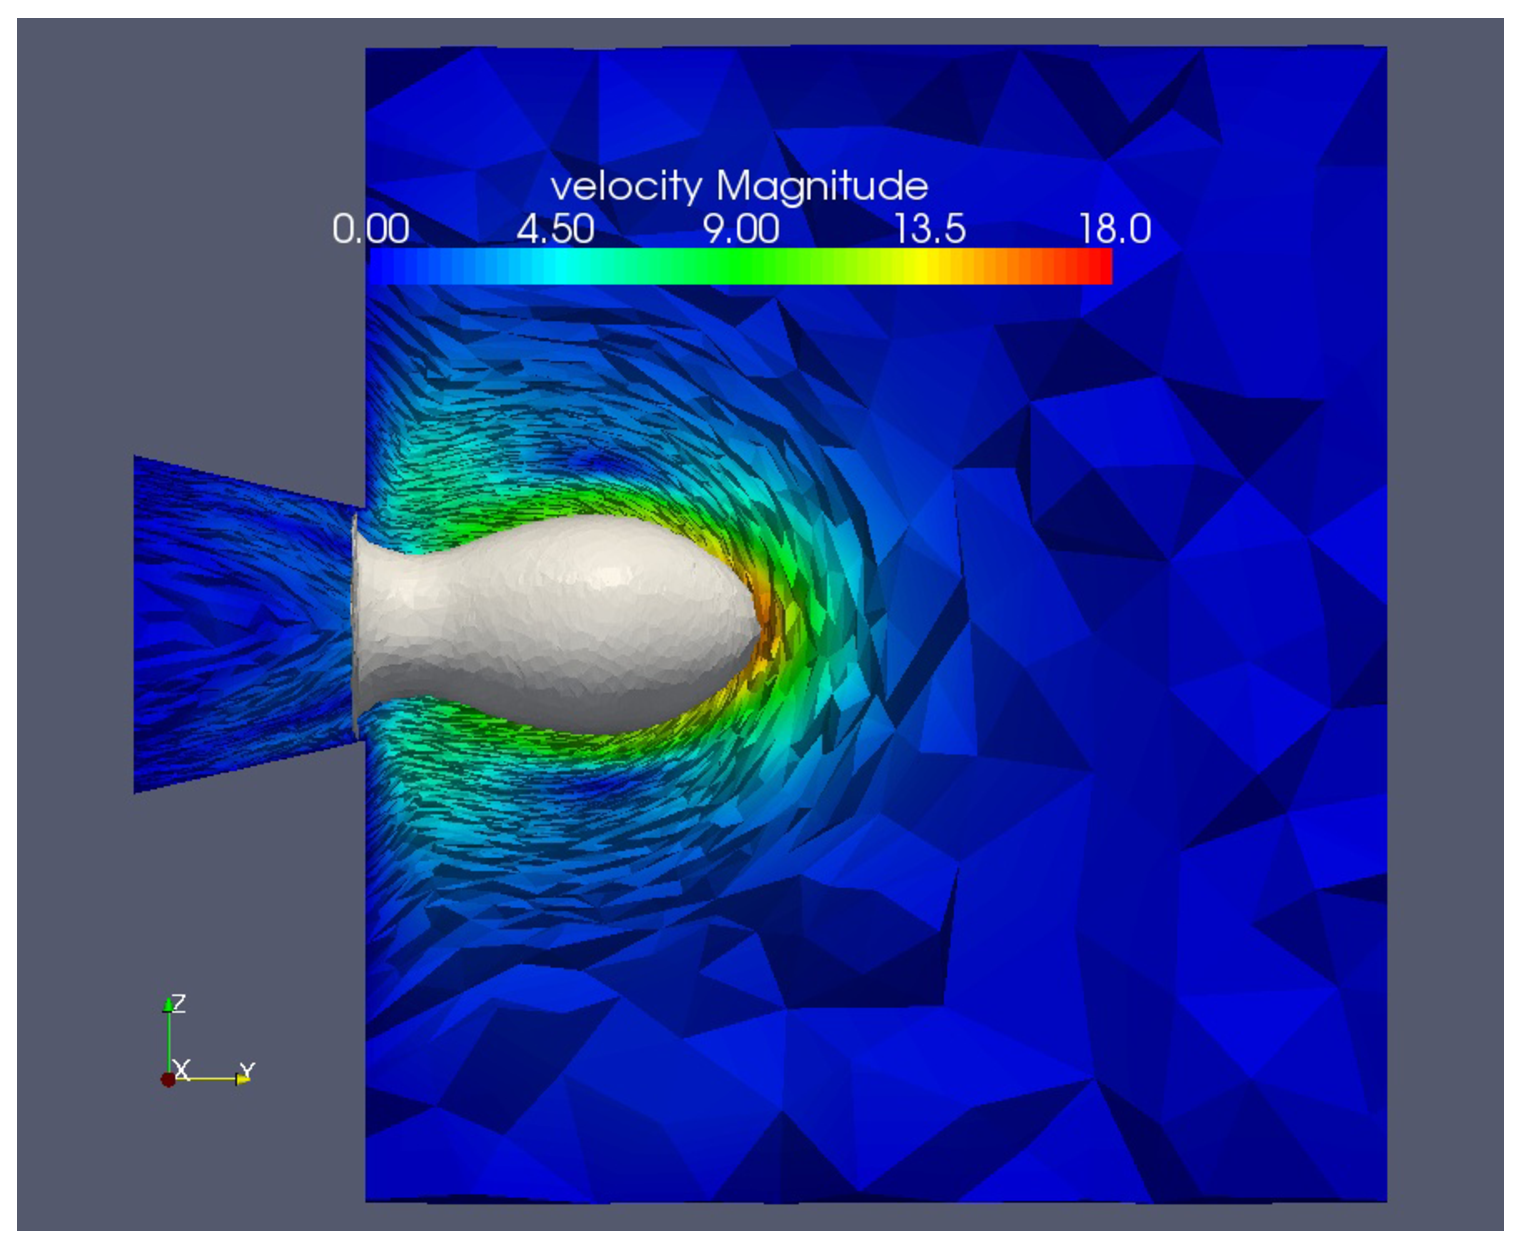
\includegraphics[width=0.49\textwidth]{figures/fig2d.eps}
  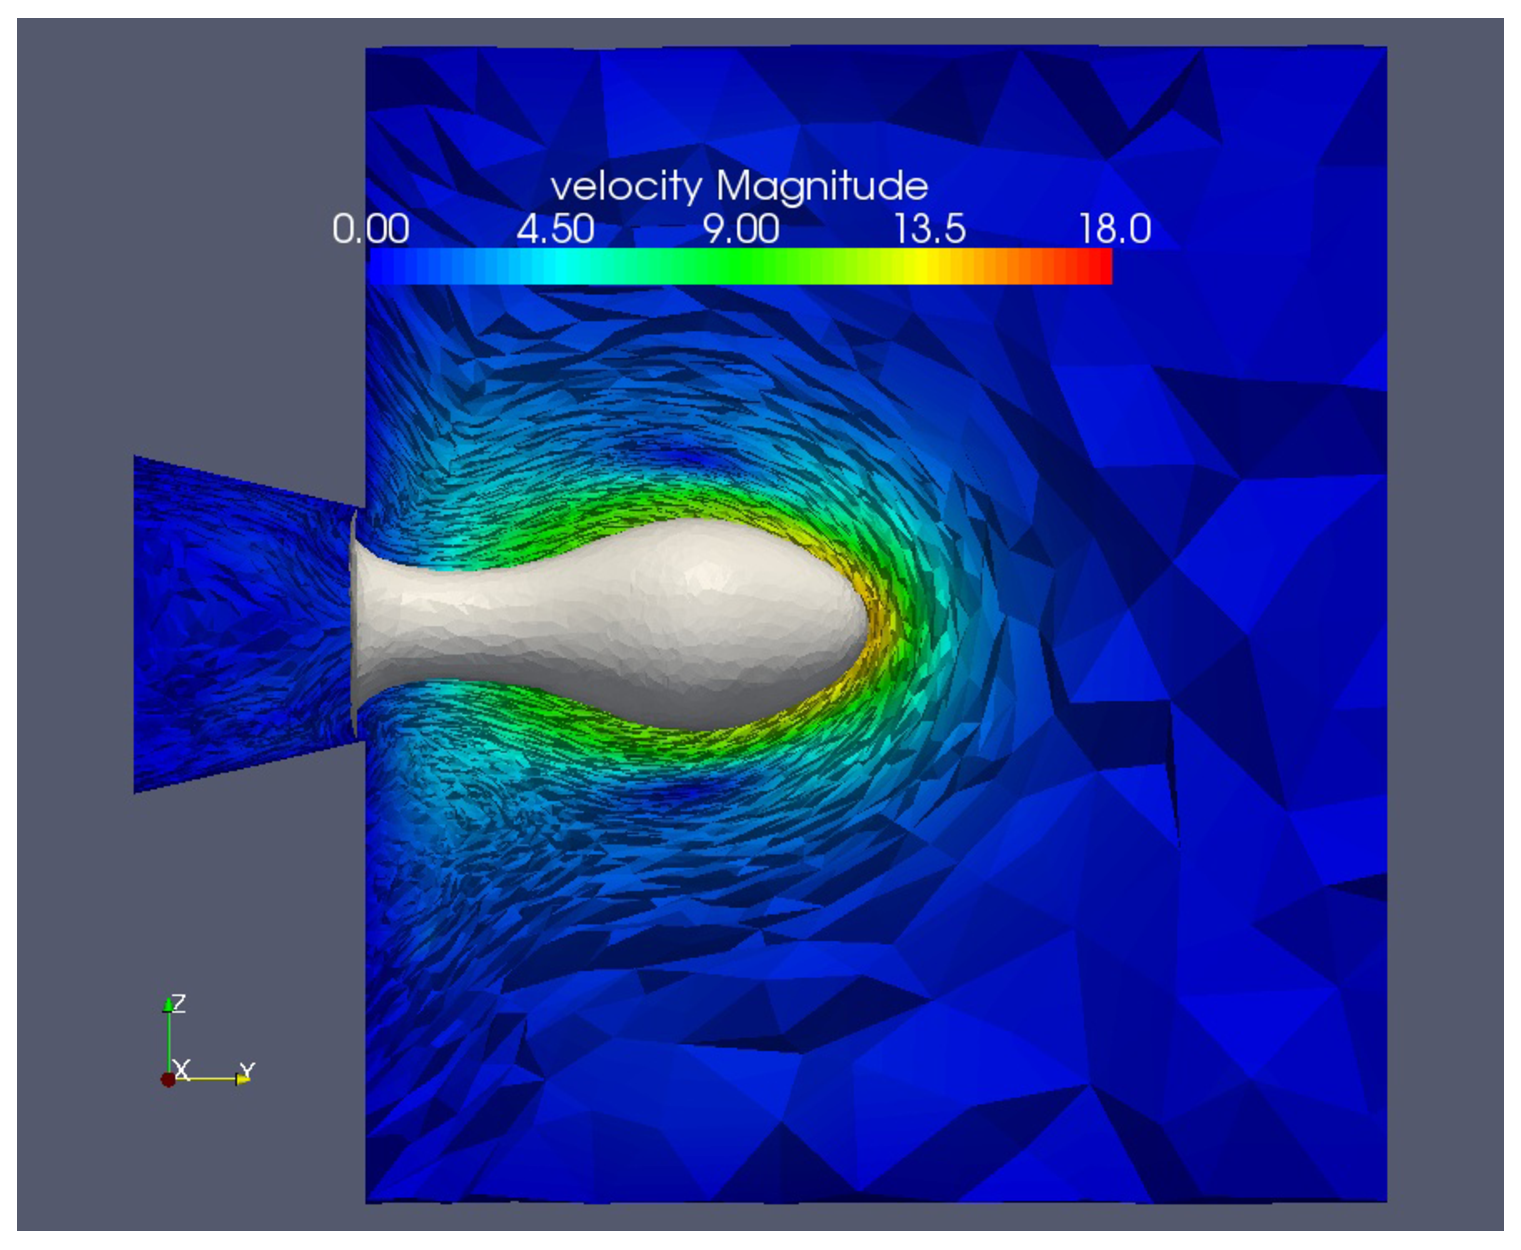
\includegraphics[width=0.49\textwidth]{figures/fig2e.eps}
  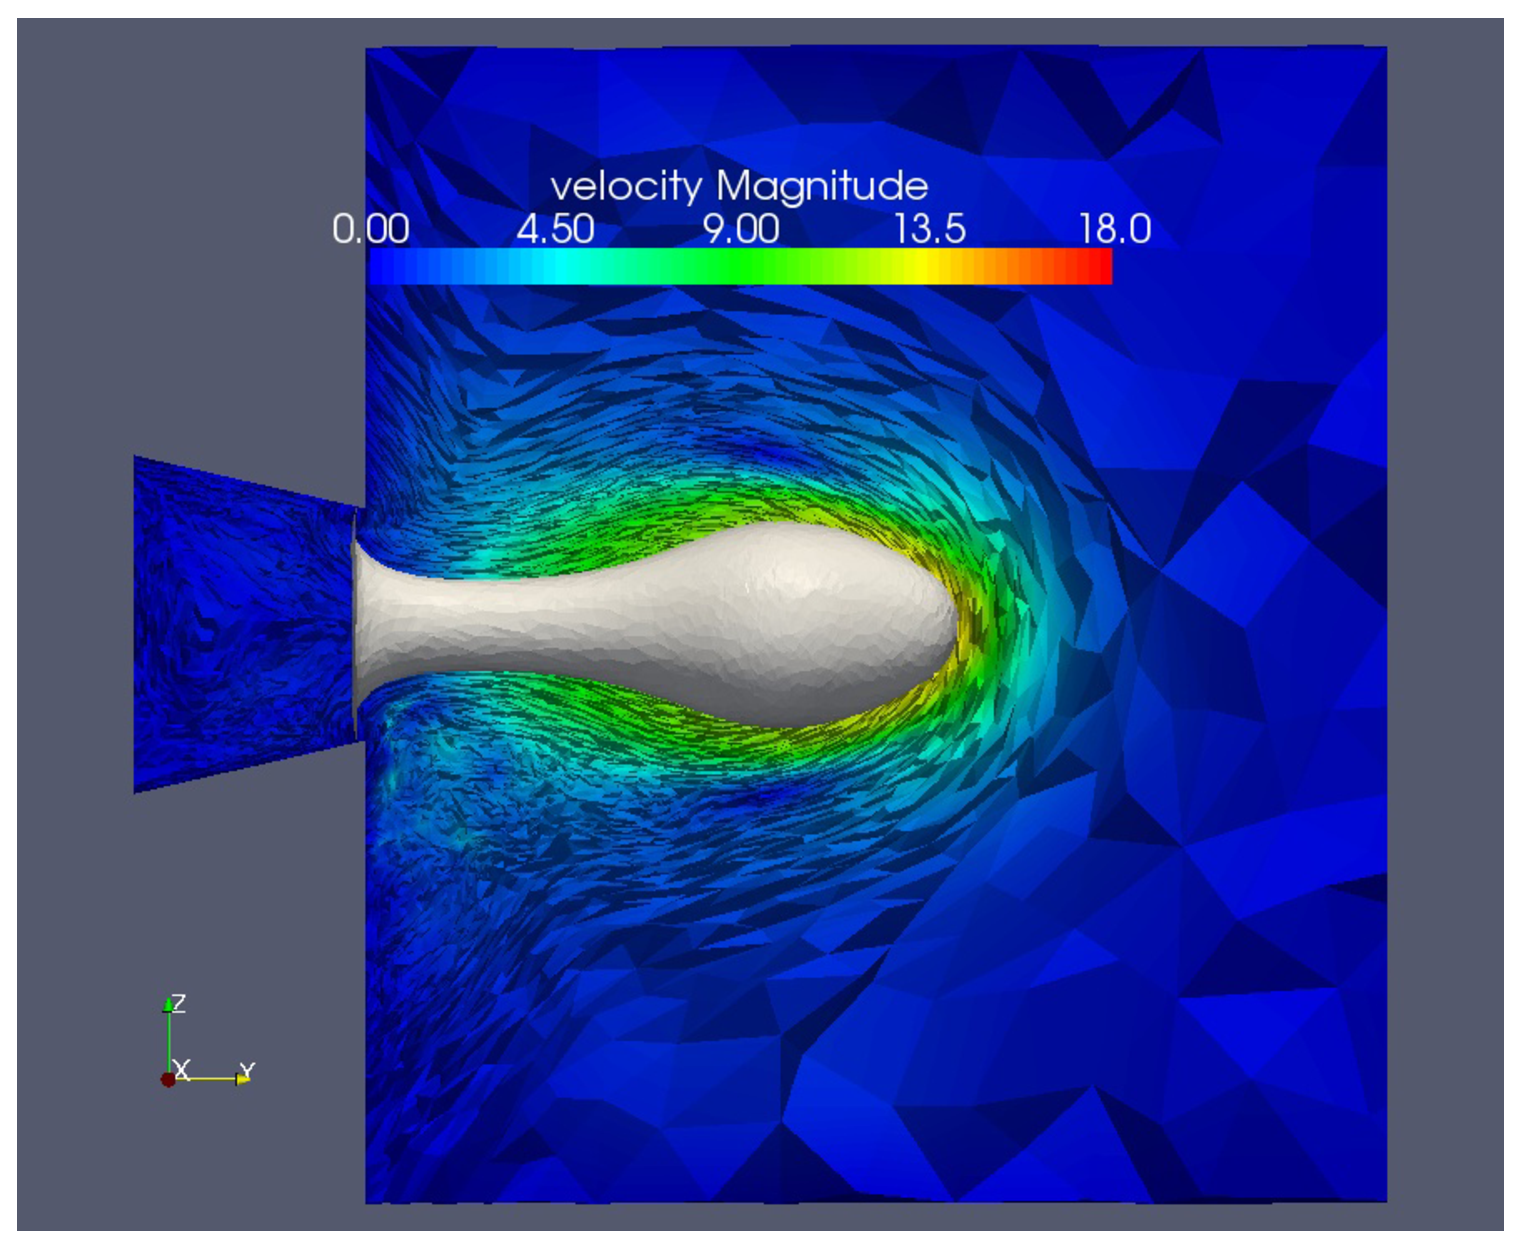
\includegraphics[width=0.49\textwidth]{figures/fig2f.eps}
  \caption{
    An axial slice of the 3D mesh at six consecutive adaptation cycles in the
    multi-phase PHASTA simulation (top to bottom, left to right).
    The gray surface is the phasic interface.
  }
  \label{fig:micromech}
\end{figure}

Modifications to the PHASTA parallel fluid dynamics simulation software
were required to couple it to the structural mechanics code
provided by the device engineers.
To support these interactions mechanisms were implemented that interpolate
fields between the different time and spatial discretizations .
Modifications were also made to the PHASTA error estimator to reduce
discretization error and reduce computational costs.
At the phasic interface, where there is a change in material properties, the
mesh is refined.
Away from the interface, the mesh is coarsened to reduce computational costs.
Between the refined and coarse zones the mesh smoothly transitions between
the two sizes~\cite{chitale2014anisotropic,Sahn06}.
Fig.~\ref{fig:micromech} depicts the mesh over six adaptation cycles.
Simulations using this workflow were run on up to 512 processors of a CCI
cluster.
Increased scalability of this workflow is now possible through the in-memory
coupling of the PHASTA analysis component with the PUMI mesh
adaptation and load balancing components described in
Section~\ref{sec:imp_phasta}.
This scalable workflow enables device engineers to leverage HPC resources to
run high fidelity system simulations in hours instead of days, and thus reduce
the time required to develop a new device.

\section{High-fidelity Viscous Flow Simulation}\label{sec:twinscrew}

The second industrial flow problem to demonstrate component-based simulation
workflows is a non-Newtonian viscous flow in a twin-screw extruder.
The material flow of interest exhibits highly nonlinear behavior (e.g.,
follows generalized non-Newtonian constitutive law) along with nonlinear partial
slip at the screw surfaces.
Simulations support studying the processing performance of these materials
within extruder systems that are designed with thin gaps between adjacent screws
(e.g., twin-screw extrusion) and with passage walls.

The PHASTA CFD analysis component was selected for these simulations
due to our extensive experience with it, its support for non-Newtonian material
models~\cite{marrero2014numerical,phastaPartialSlip2014}, non-linear partial
slip boundary conditions, and scalability.
PHASTA inputs are created with the chef pre-processing tool using meshes
generated with Simmetrix MeshSim~\cite{simmodsuite}.
Twin screw extuder meshes produced by MeshSim have automatically generated layered
element structures that span thin section gaps and unstructured tetrahedron away
from the gaps.

The geometry of the extruder is composed of complex curved surfaces with
corners and thin gaps at which critical physics occurs.
High aspect-ratio semi-structured boundary layer meshes are constructed over
these complex surfaces, including in thin gaps, and appropriately graded into
the general unstructured mesh in the remainder of the domain.
The mesh, and axial velocity of the flow, is shown in
Fig.~\ref{fig:tseMeshAndFlow} across two threads and an axial section.
For this problem with multiple threads of the screw and tighter gaps, meshes can
range from 20 to 50 millions elements in order to obtain accurate solution.
In-turn, to obtain the solution in a reasonable time frame, less than a few hours,
the PHASTA flow analysis requires on the order of 500 cores.

\begin{figure} \centering
  \includegraphics[height=4.5cm,keepaspectratio]{figures/tseMeshTwoThreads.png}
  \includegraphics[height=4.5cm,keepaspectratio]{figures/tseMeshCrossSection.png}
  \includegraphics[height=4.5cm,keepaspectratio]{figures/tseFlowTwoThreads.png}
  \includegraphics[height=4.5cm,keepaspectratio]{figures/tseFlowCrossSection.png}
  \caption{
    Twin-screw extruder (left) mesh and (right) axial velocity: (sub-left) two
    threads of the screw and (sub-right) cross-section of the extruder.
  }
  \label{fig:tseMeshAndFlow}
\end{figure}

It should be noted that while these research efforts were being pursued
computational scientists also worked with the industrial partner's domain experts
to support their sub-continuum modeling efforts.
These researchers and engineers had experience using the computational tools,
but needed assistance installing and optimizing them for the Rensselaer Blue
Gene/Q system.
Performance tuning identified installation options, problem sizes, and run time
environment options that increased simulation efficiency of the
\textit{ab initio} packages VASP and GROMACS, and the molecular statics/dynamics
package LAMMPS.

Science domain experts are often proficient in the multiple aspects of remotely
executing jobs on large parallel systems.
Despite this apparent proficiency, they spend significant time overcoming problems that
would be trivial for a systems programming expert.
Furthermore, the solutions to said problems are often not aligned with best
practices.
Clearly, training is one path to recover productivity and increase skills in
related critical areas (such as reproducibility and data management) but there
is another approach.
Web-based science gateways let a small team of system and programming experts
create workflows for execution on multiple different remote systems without
burdening the domain experts with details of each system.
For the domain experts, they simply use a web-browser to upload their input data,
set simulation control parameters, choose a parallel system to execute on and
the level of parallelism, then submit the job.
When execution completes the outputs are made available for download.

We have built a science gateway to support PHASTA
users~\cite{phasta_gateway}.
A science gateway is a community-developed set of tools, applications, and data
collections that are integrated through a portal or a suite of applications.
These gateway technologies support PHASTA workflows on HPC systems while
hiding complexities such as data management, job scheduling, and
run-time environment setup.
The PHASTA science gateway was created using the PHP Reference Gateway
for Airavata (PGA)~\cite{airavata2011,scigap2014,airavata2015} and is hosted in
the XSEDE gateway hosting environment.
PGA is a general-purpose gateway framework developed to enable scientific
application in a browser environment.
It provides user management, application cataloging and experiment management.

The PHASTA partial-slip workflow described in the previous section, and the
in-memory adaptive workflow of Section~\ref{sec:imp_phasta}, were implemented
with two PGA Application Modules.
Each module acts as a hub to associate workflow inputs and outputs (Application
Interfaces) with the execution mechanisms (Deployments).
For the partial-slip workflow the Deployment executes the serial pre-processing
executable, followed by execution of the PHASTA binary with support for
the necessary non-Newtonian fluid model and partial-slip boundary conditions.
The in-memory workflow has two Deployments associated with it; one for execution
of the PHASTA-chef binary on the TACC Stampede Xeon host processors and
another for the Stampede KNL nodes.
Fig.~\ref{fig:phastaGatewayOrg} depicts these associations.

\begin{figure} \centering
  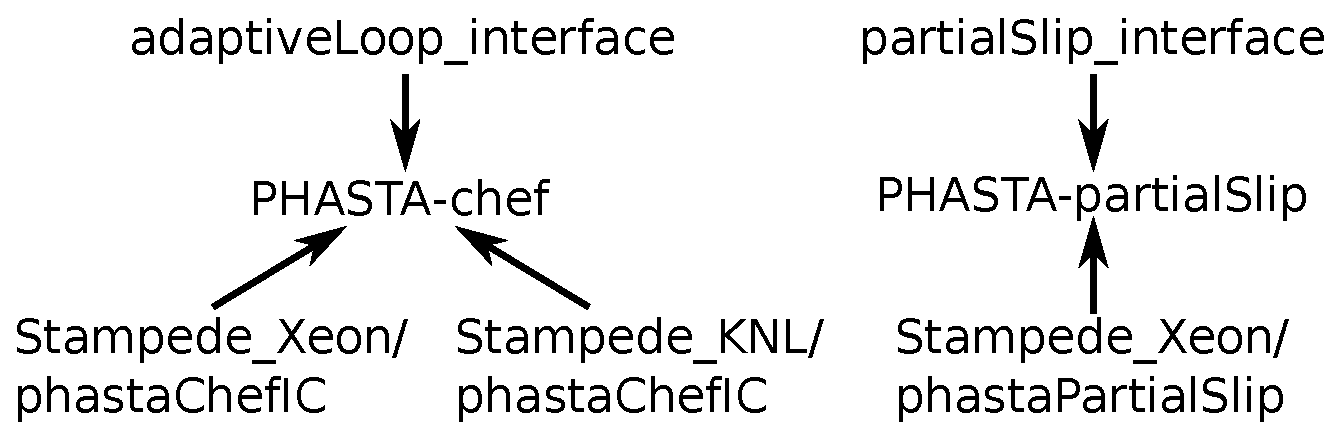
\includegraphics[width=0.6\textwidth]{figures/phastaGatewayOrg.eps}
  \caption{
    PGA (top) Application Interfaces, (middle) Modules, and (bottom) Deployments defined for
    the PHASTA gateway workflows.
  }
  \label{fig:phastaGatewayOrg}
\end{figure}

Simulations, called ‘experiments’ in the gateway, are defined by uploading a set
of input files that specify the problem definition, simulation parameters, and
required compute resources.
The left half of Fig.~\ref{fig:createExperiment} depicts the experiment
creation interface.
The application inputs include the complete definition of the analysis
domain via the geometric model (typically from a CAD software such as
SolidWorks, NX, etc.) and the unstructured mesh.
Also, included are information associated geometric model entities, such as
physical attribute information (e.g., loads, boundary conditions, material
properties) and simulation parameters (e.g., initial mesh control, time steps,
convergence requirements, solver options, etc.).
Lastly, the compute resource inputs specify the HPC system, TACC’s Stampede
system for this example, the node and core count, and the maximum run time.

Once the experiment is defined, clicking the ‘Save and launch’ button shown in
the left half of Fig.~\ref{fig:createExperiment} will execute the PHASTA workflow.
The experiment execution request is supported through APIs provided by SciGaP
~\cite{scigap2014}.
SciGaP APIs process the user request, create a job scheduler script specific to
a compute resource (PBS, SLURM, etc.), and monitor the status of a job, as shown
in the right half of Fig.~\ref{fig:createExperiment}.
SciGaP also supports email notifications triggered by job status changes; an
important mechanism for effective interactions with scheduled HPC systems.
At the end of an experiment, the SciGaP service moves the outputs to the PGA
storage location for users to download.

\begin{figure} \centering
  \includegraphics[height=0.7\textheight,keepaspectratio]{figures/createExperiment.png}
  \includegraphics[height=0.4\textheight,keepaspectratio]{figures/experimentSummary.png}
  \caption{
    PHASTA gateway experiment creation and management interface.
  }
  \label{fig:createExperiment}
\end{figure}

\section{Semi-automated Pump Design}\label{sec:pumpdesign}

Hydraulic engineers at a New York State pump manufacturer study pump design over
a range of operating conditions with the goal of developing an optimum pump
configuration and geometry.
Parallel CFD simulations provide a cost effective
way to study the performance.
One critical factor for providing competitive advantage is reducing the time
needed to set up and run simulations.
Since an ensemble of simulations are needed to cover the design space, a
vast majority of the engineers' time is spent in simulation set up.
Therefore, Rensselaer computational scientists worked with Simmetrix software
engineers to define an automated workflow for setting up the ensembles.
Setting up a simulation entails association of mesh generation controls and problem
definition attributes with the geometric model, mesh generation, and creation of
the CFD analysis software inputs.

The workflow depicted in Fig.~\ref{fig:pumps} combines customizations to the
Simmetrix and ANSYS tools for semi-automated set up and execution of an ensemble
of \mbox{ANSYS} CFX~\cite{ansysCFX} parallel simulations.
Phase 1 of the workflow uses the Simmetrix AbstractModel
component~\cite{simmodsuite,simmetrixAbstractModel}, mesh size control
attributes, and a custom set of Attribute Definitions to support user creation
of a problem template.
The template defines the association of AbstractModel components
representing features of the geometric model with the mesh and problem
definition attributes.
For example, the geometric model features of an impeller includes the blade,
inlet, outlet, hub, and shroud surfaces.
In the impeller template an inflow boundary condition will be associated with
the inlet surface, a no-slip condition with the hub, blade and shroud surfaces,
and an outflow condition on the outlet surface.
Likewise, size gradation, boundary layer, curvature refinement mesh generation
controls can be associated with the AbstractModel components.

\begin{figure} \centering
  \includegraphics[width=\textwidth]{figures/pumpAbstractModelWorkflowSummary.jpg}
  \caption{
    Workflow from abstraction to simulation~\cite{simmodsuite}.
  }
  \label{fig:pumps}
\end{figure}

Custom Attribute Definitions define the sets of information needed to create
boundary conditions, initial conditions, material properties, and simulation
control parameters to drive ANSYS CFX two-phase simulations.
Fig.~\ref{fig:inletAttribute} depicts the SimModeler interface for the inlet
attribute and Listing~\ref{lst:inletAttributeDef} shows a snippet of the code
that defines it.
In the graphical interface the geometric model associations are listed at the
bottom with required fields listed above.
The depicted inlet boundary condition is created by the derived boundary
condition type specified on Line 3 of the Attribute Definition code.
Its parent type specification on Line 1 defines the possible
geometric model entity dimensions (face, edge or vertex \texttt{< f e v >})
that the derived inlet type can be associated with.
Fields required for specifying the inlet types `flow direction' are listed on
Lines 5 through 14.
Using the parent and derived type mechanism, three options are provided to
users.
The \texttt{cartesian} option requires a one dimensional tensor
of length three ($l.$7, \texttt{tensor1 3}) while the \texttt{cylindrical} flow
direction specification requires one double ($l.$11-13, \texttt{double}) for
each of the axial, radial and theta coordinate components.
Using this syntax and similar constructs the full set of problem definition
attributes are defined.
The attributes and their organization through the type mechanism are defined
following a layout that mirrors the CFX interface; the challenges of teaching
engineers a new set of tools and processes is difficult enough without
complicating it with sweeping interface changes.


\begin{figure} \centering
  \includegraphics[width=0.45\textwidth]{figures/simModelerInletBC.png}
  \caption{
    Custom attribute definition interface for the inlet boundary
    condition.
  }
  \label{fig:inletAttribute}
\end{figure}

\begin{lstlisting}[
  float,
  escapeinside=||,
  label=lst:inletAttributeDef,
  caption=A snippet of the Attribute Definition code defining
            the inlet attribute shown in Fig.~\ref{fig:inletAttribute}.]
  |
  \centering
     \includegraphics[width=0.8\textwidth]{figures/boundaryConditionAttDef.png}
  |
\end{lstlisting}

Phase 2 of Fig.~\ref{fig:pumps} combines tagged geometric model
instances (i.e., identification strings associated with geometric model
entities) with the templates defined in Phase 1 to create fully attributed
geometric models.
Each model is then meshed in Phase 3 and CFX analysis input decks are created.
Each input deck is composed of a mesh, in a FLUENT format, and the CFX
analysis definition file (.ccl).
The analysis file is created using a custom Simmetrix SimModSuite Export
Pattern.
The portion of the CFX Export Pattern code for writing the inlet boundary
condition's flow direction information to the analysis definition input file is
shown in Listing~\ref{lst:inletExport}.
On Line 1 is a loop over all the geometric model faces with \texttt{boundary
condition} attributes associated with them.
Lines 6, 19 and 27 respectively process the three derived types for the flow
direction.
Within the blocks for the \texttt{components} and \texttt{cylindrical} derived
types are formatted strings containing the tensor ($l.$13-15) and
double precision ($l.$22-24) values.
These strings are in turn written to the precious \texttt{header} variable which
is flushed to the CFX analysis definition file.

\begin{lstlisting}[
  float,
  escapeinside=||,
  label=lst:inletExport,
  caption=A portion of the Export Pattern code for writing the inlet boundary
          condition flow direction information to the ANSYS CFX analysis input file.]
  |
  \centering
    \includegraphics[width=0.8\textwidth]{figures/boundaryConditionExport.png}
  |
\end{lstlisting}

In Phase 4 of Fig.~\ref{fig:pumps} the user loads the CFX analysis input and Fluent
mesh into ANSYS Workbench along with a table of design points.
Each design point defines values for selected boundary conditions to drive an
ensemble of simulations that covers the design space.
Each design point simulation is then executed on a cluster using one of the
natively supported job schedulers or our custom integration of the ANSYS Remote
Solver Manager with the open-source job scheduler SLURM~\cite{slurm2003}.

Hydraulic engineers using this workflow bypass many tedious and error prone steps.
This automation increases their time spent on design and analysis, which results
in better products.
Using an early version of this process helped bring a heavy-duty pump to market
which later won industry product awards.

